% Options for packages loaded elsewhere
\PassOptionsToPackage{unicode}{hyperref}
\PassOptionsToPackage{hyphens}{url}
\PassOptionsToPackage{dvipsnames,svgnames,x11names}{xcolor}
%
\documentclass[
  letterpaper,
  DIV=11,
  numbers=noendperiod]{scrreprt}

\usepackage{amsmath,amssymb}
\usepackage{iftex}
\ifPDFTeX
  \usepackage[T1]{fontenc}
  \usepackage[utf8]{inputenc}
  \usepackage{textcomp} % provide euro and other symbols
\else % if luatex or xetex
  \usepackage{unicode-math}
  \defaultfontfeatures{Scale=MatchLowercase}
  \defaultfontfeatures[\rmfamily]{Ligatures=TeX,Scale=1}
\fi
\usepackage{lmodern}
\ifPDFTeX\else  
    % xetex/luatex font selection
\fi
% Use upquote if available, for straight quotes in verbatim environments
\IfFileExists{upquote.sty}{\usepackage{upquote}}{}
\IfFileExists{microtype.sty}{% use microtype if available
  \usepackage[]{microtype}
  \UseMicrotypeSet[protrusion]{basicmath} % disable protrusion for tt fonts
}{}
\makeatletter
\@ifundefined{KOMAClassName}{% if non-KOMA class
  \IfFileExists{parskip.sty}{%
    \usepackage{parskip}
  }{% else
    \setlength{\parindent}{0pt}
    \setlength{\parskip}{6pt plus 2pt minus 1pt}}
}{% if KOMA class
  \KOMAoptions{parskip=half}}
\makeatother
\usepackage{xcolor}
\setlength{\emergencystretch}{3em} % prevent overfull lines
\setcounter{secnumdepth}{5}
% Make \paragraph and \subparagraph free-standing
\ifx\paragraph\undefined\else
  \let\oldparagraph\paragraph
  \renewcommand{\paragraph}[1]{\oldparagraph{#1}\mbox{}}
\fi
\ifx\subparagraph\undefined\else
  \let\oldsubparagraph\subparagraph
  \renewcommand{\subparagraph}[1]{\oldsubparagraph{#1}\mbox{}}
\fi

\usepackage{color}
\usepackage{fancyvrb}
\newcommand{\VerbBar}{|}
\newcommand{\VERB}{\Verb[commandchars=\\\{\}]}
\DefineVerbatimEnvironment{Highlighting}{Verbatim}{commandchars=\\\{\}}
% Add ',fontsize=\small' for more characters per line
\usepackage{framed}
\definecolor{shadecolor}{RGB}{241,243,245}
\newenvironment{Shaded}{\begin{snugshade}}{\end{snugshade}}
\newcommand{\AlertTok}[1]{\textcolor[rgb]{0.68,0.00,0.00}{#1}}
\newcommand{\AnnotationTok}[1]{\textcolor[rgb]{0.37,0.37,0.37}{#1}}
\newcommand{\AttributeTok}[1]{\textcolor[rgb]{0.40,0.45,0.13}{#1}}
\newcommand{\BaseNTok}[1]{\textcolor[rgb]{0.68,0.00,0.00}{#1}}
\newcommand{\BuiltInTok}[1]{\textcolor[rgb]{0.00,0.23,0.31}{#1}}
\newcommand{\CharTok}[1]{\textcolor[rgb]{0.13,0.47,0.30}{#1}}
\newcommand{\CommentTok}[1]{\textcolor[rgb]{0.37,0.37,0.37}{#1}}
\newcommand{\CommentVarTok}[1]{\textcolor[rgb]{0.37,0.37,0.37}{\textit{#1}}}
\newcommand{\ConstantTok}[1]{\textcolor[rgb]{0.56,0.35,0.01}{#1}}
\newcommand{\ControlFlowTok}[1]{\textcolor[rgb]{0.00,0.23,0.31}{#1}}
\newcommand{\DataTypeTok}[1]{\textcolor[rgb]{0.68,0.00,0.00}{#1}}
\newcommand{\DecValTok}[1]{\textcolor[rgb]{0.68,0.00,0.00}{#1}}
\newcommand{\DocumentationTok}[1]{\textcolor[rgb]{0.37,0.37,0.37}{\textit{#1}}}
\newcommand{\ErrorTok}[1]{\textcolor[rgb]{0.68,0.00,0.00}{#1}}
\newcommand{\ExtensionTok}[1]{\textcolor[rgb]{0.00,0.23,0.31}{#1}}
\newcommand{\FloatTok}[1]{\textcolor[rgb]{0.68,0.00,0.00}{#1}}
\newcommand{\FunctionTok}[1]{\textcolor[rgb]{0.28,0.35,0.67}{#1}}
\newcommand{\ImportTok}[1]{\textcolor[rgb]{0.00,0.46,0.62}{#1}}
\newcommand{\InformationTok}[1]{\textcolor[rgb]{0.37,0.37,0.37}{#1}}
\newcommand{\KeywordTok}[1]{\textcolor[rgb]{0.00,0.23,0.31}{#1}}
\newcommand{\NormalTok}[1]{\textcolor[rgb]{0.00,0.23,0.31}{#1}}
\newcommand{\OperatorTok}[1]{\textcolor[rgb]{0.37,0.37,0.37}{#1}}
\newcommand{\OtherTok}[1]{\textcolor[rgb]{0.00,0.23,0.31}{#1}}
\newcommand{\PreprocessorTok}[1]{\textcolor[rgb]{0.68,0.00,0.00}{#1}}
\newcommand{\RegionMarkerTok}[1]{\textcolor[rgb]{0.00,0.23,0.31}{#1}}
\newcommand{\SpecialCharTok}[1]{\textcolor[rgb]{0.37,0.37,0.37}{#1}}
\newcommand{\SpecialStringTok}[1]{\textcolor[rgb]{0.13,0.47,0.30}{#1}}
\newcommand{\StringTok}[1]{\textcolor[rgb]{0.13,0.47,0.30}{#1}}
\newcommand{\VariableTok}[1]{\textcolor[rgb]{0.07,0.07,0.07}{#1}}
\newcommand{\VerbatimStringTok}[1]{\textcolor[rgb]{0.13,0.47,0.30}{#1}}
\newcommand{\WarningTok}[1]{\textcolor[rgb]{0.37,0.37,0.37}{\textit{#1}}}

\providecommand{\tightlist}{%
  \setlength{\itemsep}{0pt}\setlength{\parskip}{0pt}}\usepackage{longtable,booktabs,array}
\usepackage{calc} % for calculating minipage widths
% Correct order of tables after \paragraph or \subparagraph
\usepackage{etoolbox}
\makeatletter
\patchcmd\longtable{\par}{\if@noskipsec\mbox{}\fi\par}{}{}
\makeatother
% Allow footnotes in longtable head/foot
\IfFileExists{footnotehyper.sty}{\usepackage{footnotehyper}}{\usepackage{footnote}}
\makesavenoteenv{longtable}
\usepackage{graphicx}
\makeatletter
\def\maxwidth{\ifdim\Gin@nat@width>\linewidth\linewidth\else\Gin@nat@width\fi}
\def\maxheight{\ifdim\Gin@nat@height>\textheight\textheight\else\Gin@nat@height\fi}
\makeatother
% Scale images if necessary, so that they will not overflow the page
% margins by default, and it is still possible to overwrite the defaults
% using explicit options in \includegraphics[width, height, ...]{}
\setkeys{Gin}{width=\maxwidth,height=\maxheight,keepaspectratio}
% Set default figure placement to htbp
\makeatletter
\def\fps@figure{htbp}
\makeatother
% definitions for citeproc citations
\NewDocumentCommand\citeproctext{}{}
\NewDocumentCommand\citeproc{mm}{%
  \begingroup\def\citeproctext{#2}\cite{#1}\endgroup}
\makeatletter
 % allow citations to break across lines
 \let\@cite@ofmt\@firstofone
 % avoid brackets around text for \cite:
 \def\@biblabel#1{}
 \def\@cite#1#2{{#1\if@tempswa , #2\fi}}
\makeatother
\newlength{\cslhangindent}
\setlength{\cslhangindent}{1.5em}
\newlength{\csllabelwidth}
\setlength{\csllabelwidth}{3em}
\newenvironment{CSLReferences}[2] % #1 hanging-indent, #2 entry-spacing
 {\begin{list}{}{%
  \setlength{\itemindent}{0pt}
  \setlength{\leftmargin}{0pt}
  \setlength{\parsep}{0pt}
  % turn on hanging indent if param 1 is 1
  \ifodd #1
   \setlength{\leftmargin}{\cslhangindent}
   \setlength{\itemindent}{-1\cslhangindent}
  \fi
  % set entry spacing
  \setlength{\itemsep}{#2\baselineskip}}}
 {\end{list}}
\usepackage{calc}
\newcommand{\CSLBlock}[1]{\hfill\break\parbox[t]{\linewidth}{\strut\ignorespaces#1\strut}}
\newcommand{\CSLLeftMargin}[1]{\parbox[t]{\csllabelwidth}{\strut#1\strut}}
\newcommand{\CSLRightInline}[1]{\parbox[t]{\linewidth - \csllabelwidth}{\strut#1\strut}}
\newcommand{\CSLIndent}[1]{\hspace{\cslhangindent}#1}

\KOMAoption{captions}{tableheading}
\makeatletter
\@ifpackageloaded{tcolorbox}{}{\usepackage[skins,breakable]{tcolorbox}}
\@ifpackageloaded{fontawesome5}{}{\usepackage{fontawesome5}}
\definecolor{quarto-callout-color}{HTML}{909090}
\definecolor{quarto-callout-note-color}{HTML}{0758E5}
\definecolor{quarto-callout-important-color}{HTML}{CC1914}
\definecolor{quarto-callout-warning-color}{HTML}{EB9113}
\definecolor{quarto-callout-tip-color}{HTML}{00A047}
\definecolor{quarto-callout-caution-color}{HTML}{FC5300}
\definecolor{quarto-callout-color-frame}{HTML}{acacac}
\definecolor{quarto-callout-note-color-frame}{HTML}{4582ec}
\definecolor{quarto-callout-important-color-frame}{HTML}{d9534f}
\definecolor{quarto-callout-warning-color-frame}{HTML}{f0ad4e}
\definecolor{quarto-callout-tip-color-frame}{HTML}{02b875}
\definecolor{quarto-callout-caution-color-frame}{HTML}{fd7e14}
\makeatother
\makeatletter
\@ifpackageloaded{bookmark}{}{\usepackage{bookmark}}
\makeatother
\makeatletter
\@ifpackageloaded{caption}{}{\usepackage{caption}}
\AtBeginDocument{%
\ifdefined\contentsname
  \renewcommand*\contentsname{Table of contents}
\else
  \newcommand\contentsname{Table of contents}
\fi
\ifdefined\listfigurename
  \renewcommand*\listfigurename{List of Figures}
\else
  \newcommand\listfigurename{List of Figures}
\fi
\ifdefined\listtablename
  \renewcommand*\listtablename{List of Tables}
\else
  \newcommand\listtablename{List of Tables}
\fi
\ifdefined\figurename
  \renewcommand*\figurename{Figure}
\else
  \newcommand\figurename{Figure}
\fi
\ifdefined\tablename
  \renewcommand*\tablename{Table}
\else
  \newcommand\tablename{Table}
\fi
}
\@ifpackageloaded{float}{}{\usepackage{float}}
\floatstyle{ruled}
\@ifundefined{c@chapter}{\newfloat{codelisting}{h}{lop}}{\newfloat{codelisting}{h}{lop}[chapter]}
\floatname{codelisting}{Listing}
\newcommand*\listoflistings{\listof{codelisting}{List of Listings}}
\makeatother
\makeatletter
\makeatother
\makeatletter
\@ifpackageloaded{caption}{}{\usepackage{caption}}
\@ifpackageloaded{subcaption}{}{\usepackage{subcaption}}
\makeatother
\ifLuaTeX
  \usepackage{selnolig}  % disable illegal ligatures
\fi
\usepackage{bookmark}

\IfFileExists{xurl.sty}{\usepackage{xurl}}{} % add URL line breaks if available
\urlstyle{same} % disable monospaced font for URLs
\hypersetup{
  pdftitle={Computational Statistics},
  pdfauthor={Nina Leach},
  colorlinks=true,
  linkcolor={blue},
  filecolor={Maroon},
  citecolor={Blue},
  urlcolor={Blue},
  pdfcreator={LaTeX via pandoc}}

\title{Computational Statistics}
\author{Nina Leach}
\date{}

\begin{document}
\maketitle

\renewcommand*\contentsname{Table of contents}
{
\hypersetup{linkcolor=}
\setcounter{tocdepth}{2}
\tableofcontents
}
\bookmarksetup{startatroot}

\chapter*{Preface}\label{preface}
\addcontentsline{toc}{chapter}{Preface}

\markboth{Preface}{Preface}

\part{Probability}

The following uses Pishro-Nik (2014)

\section*{Random Variables}\label{random-variables}
\addcontentsline{toc}{section}{Random Variables}

\markright{Random Variables}

A random experiment is a procedure where uncertain events are observed.
An \textbf{outcome} is the result of such an experiment, and the
collection of all possible outcomes is called the \textbf{sample space}
\(S\). For example:

\begin{itemize}
\item
  a coin toss: \(S = \{heads,tails\}\)
\item
  roll a 6 sided die (D6): \(S = \{1, 2, 3, 4, 5, 6\}\)
\item
  number of rainy days in June: \(S = \{0, 1, ..., 30\}\)
\end{itemize}

Repetitions of a random experiment is known as a \textbf{trial.} If a
coin is tossed twice \(S = \{(H, H), (T, H), (H, T), (T, T)\}\).

An \textbf{event} is a subset of the sample space.

The numerical results of an a random experiment are \textbf{random
variables(RV)}. For the example of a coin tossed twice, numeral values
can be assigned to each outcome: \((H, H) = 0, (T, H) = 1, ...\)

The set of possible values for random variable \(X\) is denoted by
\(Range(X)\), \(R_X\), \(\Omega\).

\begin{enumerate}
\def\labelenumi{\arabic{enumi}.}
\item
  I roll a D6 10 times. Let X be the number of 1's observed. Then
  \(R_X = \{0, 1, ..., 10\}\)
\item
  How many attempts it takes for Manchester United (F.C.) defense to
  tighten up. Let Y represent the total number of games before they
  manage to keep a clean sheet. Then
  \(R_Y = \{ 1,2, ...\} = \mathbb{N}\) i.e.~Y can be any positive
  integer.
\item
  The random variable T is the time (in hours) from now until the next
  earthquake occurs. This can be any non negative real number
  \(R_T = [0, \infty)\)
\end{enumerate}

\part{}

\chapter{Discrete random variables}\label{discrete-random-variables}

A random variable X is called discrete if:

\begin{enumerate}
\def\labelenumi{\arabic{enumi}.}
\item
  \(\Omega\) is a finite set. E.g. \(\Omega_X = \{1, 2, 3, 4\}\).
\item
  a countably infinite set. E.g.:

  \begin{itemize}
  \item
    Natural numbers \(\mathbb{N} = \{1, 2, 3, ...\}\),
  \item
    Integers \(\mathbb{Z} = \{..., -1, 0, 1,...\}\),
  \item
    \textbf{Rational number}, \(\mathbb{Q}\) (number that can be
    expressed as a fraction), etc..
  \end{itemize}
\end{enumerate}

If \(\Omega\) isn't a countable set, X is continuous.

\subsection{Definitions explained through an
example}\label{definitions-explained-through-an-example}

If a coin is tossed four times:

\begin{itemize}
\item
  The sample space (S) ---the list of all (\(2^4\)) possible outcomes---
  is \(S = \{(H, H, H, H), (H, H, H, T), ....\}\).
\item
  We define the RV, \(X\), as the number of heads that come up in the
  four coin tosses. Then the range of X is
  \(\Omega_X = \{x_1 = 0, x_2 = 1,..., x_5= 4\}\).
\item
  An \textbf{event} defined as the set of outcomes \textbf{\emph{s}} in
  the sample space \textbf{\emph{S}}. For example an event, \textbf{A},
  could be ``getting exactly 2 heads''. Then \textbf{A} would include
  all outcomes from the sample space where there are 2 heads, e.g.:
  \((HHTT), (HTHT),\) etc. In general terms \(A=\{s∈S|X(s)=x_k\}\)
\item
  Probabilities of events \(\{X=x_k\}\) are formally shown by the
  probability mass function (\textbf{pmf}) of \(X\), i.e.~showing the
  probability of each value of \(\Omega_X\): \(P(X=0), ..., P(X=4)\).
  Formally, the \textbf{pmf}: \(f_X(x_k) = P(X=x_k)\).
\end{itemize}

\begin{figure}

\centering{

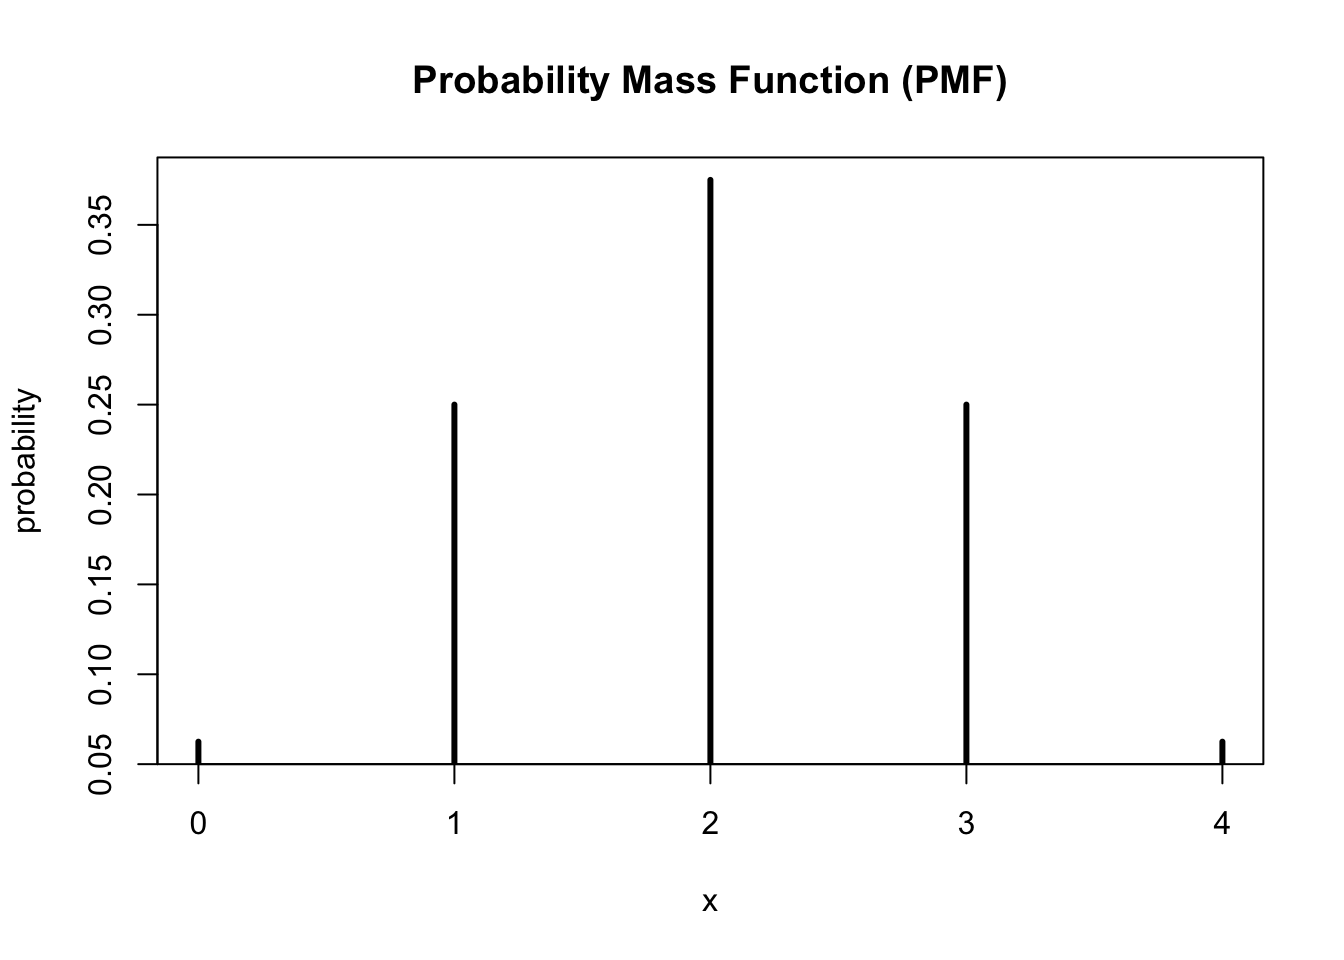
\includegraphics{discreteRV_files/figure-pdf/fig-coin_pmf1-1.pdf}

}

\caption{\label{fig-coin\_pmf1}e.g.~P(X = 1): The probability of getting
1 head (HTTT, THTT, TTHT, TTTH) = 4/(2\^{}4) = 0.25.}

\end{figure}%

\begin{itemize}
\item
  To be a pmf, \(f_X\) must have the following properties:

  \begin{itemize}
  \item
    \(f_X \ge 0\) for \(x \in \Omega\). i.e \(P(X =x_k) < 0\)
  \item
    \(\Sigma_{x \in \Omega} f_X = 1\)
  \end{itemize}

  From our example, for in each case \(f_X \ge 0\) and the sum is 1
\end{itemize}

\begin{tabular}{r|r}
\hline
Number\_of\_Heads & Probability\\
\hline
0 & 0.0625\\
\hline
1 & 0.2500\\
\hline
2 & 0.3750\\
\hline
3 & 0.2500\\
\hline
4 & 0.0625\\
\hline
\end{tabular}

\begin{itemize}
\tightlist
\item
  The \textbf{cumulative distribution function (cdf)}
  \(F_X(x) = P(X ≤ x)\)
\end{itemize}

\begin{figure}

\centering{

\captionsetup{labelsep=none}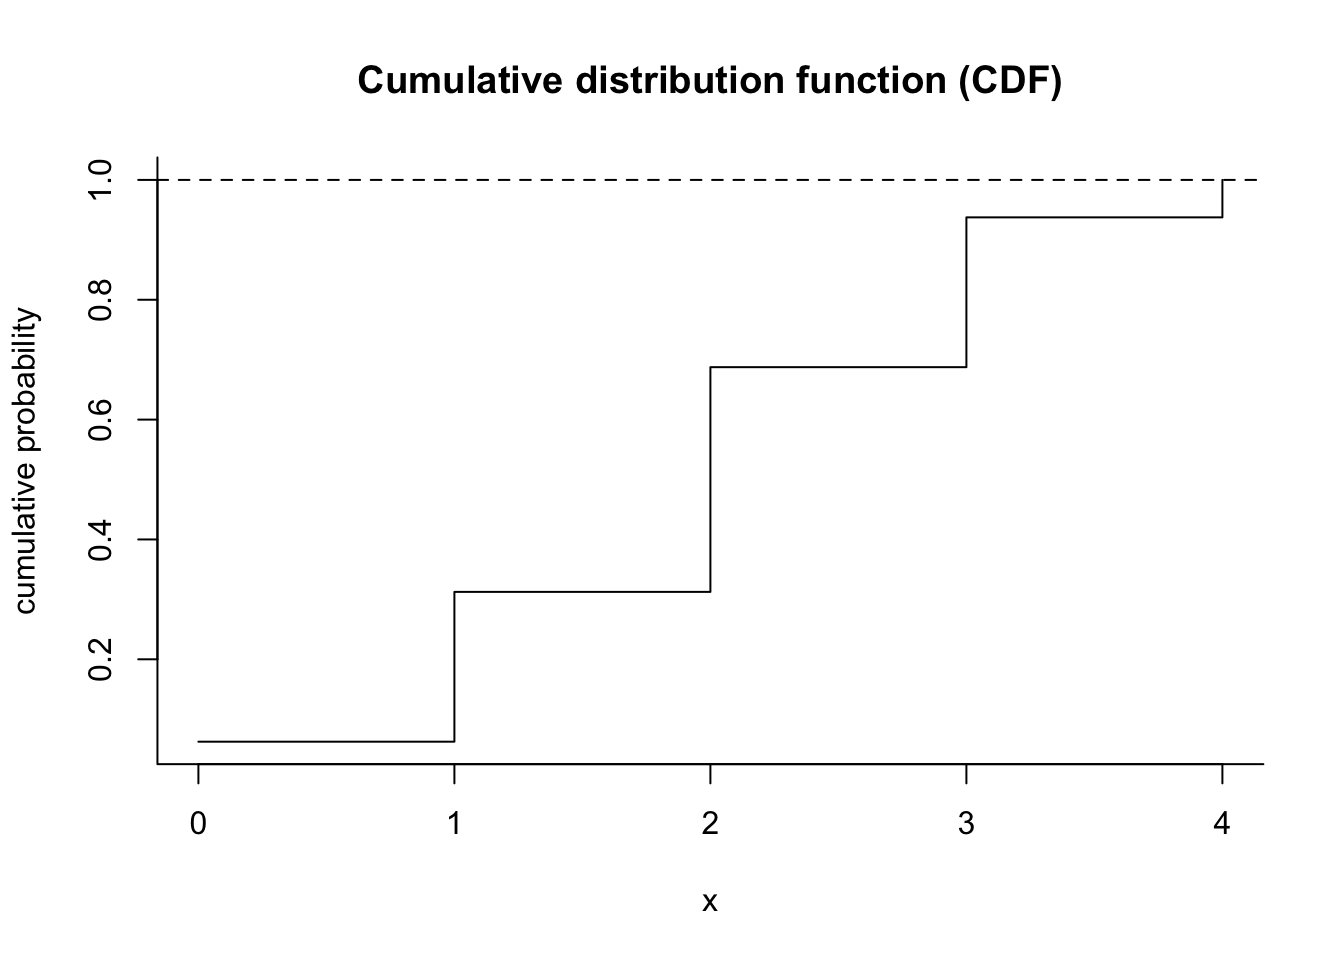
\includegraphics{discreteRV_files/figure-pdf/fig-coin_cdf-1.pdf}

}

\caption{\label{fig-coin\_cdf}}

\end{figure}%

\begin{itemize}
\tightlist
\item
  The cdf is a non-decreasing function for which
  \[\lim_{x\to - \infty} F_X(x) = 0 \text{  and } \lim_{x\to \infty} F_X(x) =1 \]
\item
  \textbf{expected value} \[E(X) = \sum_{x=\Omega} xf_X(x)\]
\item
  \textbf{variance} \[Var(X) = E[(X-E(X))^2]\]
\end{itemize}

\subsection{Examples}\label{examples}

\subsubsection{Discrete uniform
distribution}\label{discrete-uniform-distribution}

\begin{itemize}
\tightlist
\item
  flip a coin
\end{itemize}

\subsubsection{Bernoulli Distribution}\label{bernoulli-distribution}

\subsubsection{Binomial distribution}\label{binomial-distribution}

(example from Lecture 1):

Let \(Y \in \{ 0,1\}\) denote the outcome of a binary experiment. Where
a success (y=1) has probability \(p \in(0,1)\), and failure (y=0)
probability \(1-p\).

The binomial distribution \(X = \sum_{i=1}^{n} Y_i\) counts the number
of successes \(X\) out of \(n\) independent Bernoulli trials
\(Y_1, Y_2, ..., Y_n\):

\[
f_X(x) = \binom{n}{x} p^x(1 - p)^{n-x}, \quad x = 0, 1,…, n 
\]

\(E(X) = np\)

\(Var(X) = np(1 - p)\)

In R:

\begin{Shaded}
\begin{Highlighting}[]
\FunctionTok{set.seed}\NormalTok{(}\DecValTok{123}\NormalTok{)}
\NormalTok{n }\OtherTok{=} \DecValTok{7}\NormalTok{; p }\OtherTok{=} \FloatTok{0.4}
\NormalTok{omega }\OtherTok{=} \DecValTok{0}\SpecialCharTok{:}\NormalTok{n}
\NormalTok{pmf }\OtherTok{=} \FunctionTok{dbinom}\NormalTok{(}\AttributeTok{x =}\NormalTok{ omega, }\AttributeTok{size =}\NormalTok{ n, }\AttributeTok{prob =}\NormalTok{ p)}
\NormalTok{bin.distr }\OtherTok{=} \FunctionTok{data.frame}\NormalTok{(}\AttributeTok{x =}\NormalTok{ omega, pmf)}
\NormalTok{bin.distr}
\end{Highlighting}
\end{Shaded}

\begin{verbatim}
  x       pmf
1 0 0.0279936
2 1 0.1306368
3 2 0.2612736
4 3 0.2903040
5 4 0.1935360
6 5 0.0774144
7 6 0.0172032
8 7 0.0016384
\end{verbatim}

To compute the cdf

\begin{Shaded}
\begin{Highlighting}[]
\CommentTok{\# option 1}
\NormalTok{cdf1 }\OtherTok{=} \FunctionTok{pbinom}\NormalTok{(}\AttributeTok{q =}\NormalTok{ omega, }\AttributeTok{size =}\NormalTok{ n, }\AttributeTok{prob =}\NormalTok{ p)}

\CommentTok{\# option 2}
\NormalTok{cdf2 }\OtherTok{=} \FunctionTok{cumsum}\NormalTok{(pmf)}

\FunctionTok{all}\NormalTok{(}\FunctionTok{round}\NormalTok{(cdf1, }\DecValTok{10}\NormalTok{) }\SpecialCharTok{==} \FunctionTok{round}\NormalTok{(cdf2, }\DecValTok{10}\NormalTok{))}
\end{Highlighting}
\end{Shaded}

\begin{verbatim}
[1] TRUE
\end{verbatim}

Both options the same till 10 d.p.

\begin{Shaded}
\begin{Highlighting}[]
\FunctionTok{plot}\NormalTok{(bin.distr, }\AttributeTok{pch =} \DecValTok{16}\NormalTok{, }\AttributeTok{bty =} \StringTok{"l"}\NormalTok{, }\AttributeTok{col =} \StringTok{\textquotesingle{}steelblue2\textquotesingle{}}\NormalTok{,}
\AttributeTok{main =} \StringTok{\textquotesingle{}Probability mass function\textquotesingle{}}\NormalTok{)}

\FunctionTok{plot}\NormalTok{(omega, cdf1, }\AttributeTok{type =} \StringTok{\textquotesingle{}s\textquotesingle{}}\NormalTok{, }\AttributeTok{bty =} \StringTok{"l"}\NormalTok{,}
\AttributeTok{xlab =} \StringTok{\textquotesingle{}x\textquotesingle{}}\NormalTok{, }\AttributeTok{ylab =} \StringTok{\textquotesingle{}cumulative probability\textquotesingle{}}\NormalTok{,}
\AttributeTok{col =} \StringTok{\textquotesingle{}steelblue2\textquotesingle{}}\NormalTok{, }\AttributeTok{lwd =} \DecValTok{2}\NormalTok{,}
\AttributeTok{main =} \StringTok{\textquotesingle{}Cumulative distribution function\textquotesingle{}}\NormalTok{)}
\FunctionTok{abline}\NormalTok{(}\AttributeTok{h =} \DecValTok{1}\NormalTok{, }\AttributeTok{lty =} \DecValTok{2}\NormalTok{)}
\end{Highlighting}
\end{Shaded}

\begin{figure}

\begin{minipage}{0.50\linewidth}

\begin{figure}[H]

\centering{

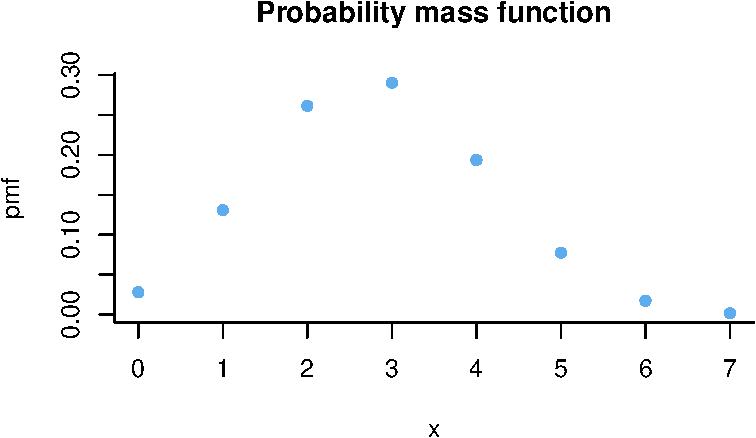
\includegraphics{discreteRV_files/figure-pdf/fig-bin.dist-1.pdf}

}

\caption{\label{fig-bin.dist-1}Corresponding PMF and CDF}

\end{figure}%

\end{minipage}%
%
\begin{minipage}{0.50\linewidth}

\begin{figure}[H]

\centering{

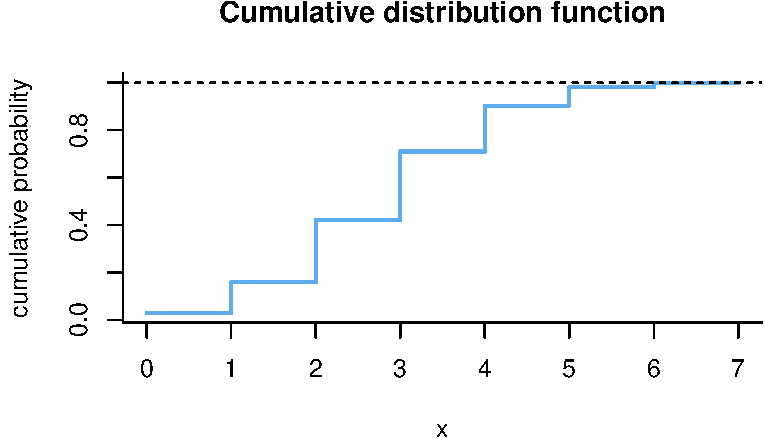
\includegraphics{discreteRV_files/figure-pdf/fig-bin.dist-2.pdf}

}

\caption{\label{fig-bin.dist-2}Corresponding PMF and CDF}

\end{figure}%

\end{minipage}%

\end{figure}%

\subsubsection{Poisson Distribution}\label{poisson-distribution}

\subsubsection{Geometric Distribution}\label{geometric-distribution}

\subsubsection{Negative Binomial (Pascal)
Distribution}\label{negative-binomial-pascal-distribution}

\subsubsection{Hypergeometric
Distribution}\label{hypergeometric-distribution}

\chapter{}\label{section-1}

\chapter{Continuous random variables}\label{continuous-random-variables}

\begin{tcolorbox}[enhanced jigsaw, bottomrule=.15mm, leftrule=.75mm, colbacktitle=quarto-callout-tip-color!10!white, toptitle=1mm, opacityback=0, titlerule=0mm, colback=white, title=\textcolor{quarto-callout-tip-color}{\faLightbulb}\hspace{0.5em}{Tip}, opacitybacktitle=0.6, left=2mm, rightrule=.15mm, breakable, bottomtitle=1mm, arc=.35mm, coltitle=black, toprule=.15mm, colframe=quarto-callout-tip-color-frame]

If ( X ) is continuous, we define:

\begin{itemize}
\item
  the probability density function (pdf) ( f\_X(x) ) as the function for
  which \[
  P(X \in A) = \int_{x \in A} f_X(t) \, dt
  \]
\item
  the cumulative distribution function (cdf) ( F\_X(x) ) \[
  F_X(x) = \int_{-\infty}^{x} f_X(t) \, dt
  \]
\item
  the expected value \[
  E(X) = \int_{-\infty}^{\infty} x f_X(x) dx
  \]
\item
  the variance \[
  Var(X) = E[(X - E(X))^2 ] \\
  Var[X] = E[X^2] - E[X]^2 \\
  \]

  Step 1:

  \[
  E[X^2] = \int_{-\infty}^{\infty} x^2 f_X(x) \, dx
  \]
\end{itemize}

\end{tcolorbox}

\subsection{Examples: Special
Distributions}\label{examples-special-distributions}

\subsubsection{Uniform}\label{uniform}

\subsubsection{Exponential}\label{exponential}

\subsubsection{Normal}\label{normal}

We say a random variable, \(X\), follows a normal distribution with mean
\(\mu\) and variance \(\sigma^2\):
\(X \sim \mathcal{N}(\mu, \sigma^2)\).

If the PDF of \(X\) is given by:

\[
f_X(x) = \frac{1}{\sigma \sqrt{2\pi}} 
  e^{-\frac{1}{2} \left(\frac{x - \mu}{\sigma}\right)^2}, 
  x \in (- \infty, \infty)
\]

In simpler terms, this formula describes how the values of the random
variable \(X\) are distributed.

example form lecture 1

\begin{Shaded}
\begin{Highlighting}[]
\FunctionTok{curve}\NormalTok{(}\FunctionTok{dnorm}\NormalTok{(x, }\AttributeTok{mean =} \DecValTok{1}\NormalTok{, }\AttributeTok{sd =} \DecValTok{1}\NormalTok{), }\AttributeTok{xlim =} \FunctionTok{c}\NormalTok{(}\SpecialCharTok{{-}}\DecValTok{4}\NormalTok{, }\DecValTok{4}\NormalTok{),}
\AttributeTok{bty =} \StringTok{\textquotesingle{}l\textquotesingle{}}\NormalTok{, }\AttributeTok{ylab =} \StringTok{\textquotesingle{}density\textquotesingle{}}\NormalTok{,}
\AttributeTok{col =} \StringTok{\textquotesingle{}steelblue2\textquotesingle{}}\NormalTok{, }\AttributeTok{lwd =} \DecValTok{2}\NormalTok{)}
\FunctionTok{abline}\NormalTok{(}\AttributeTok{v =} \DecValTok{1}\NormalTok{, }\AttributeTok{lty =} \DecValTok{2}\NormalTok{)}

\FunctionTok{curve}\NormalTok{(}\FunctionTok{pnorm}\NormalTok{(x, }\AttributeTok{mean =} \DecValTok{1}\NormalTok{, }\AttributeTok{sd =} \DecValTok{1}\NormalTok{), }\AttributeTok{xlim =} \FunctionTok{c}\NormalTok{(}\SpecialCharTok{{-}}\DecValTok{4}\NormalTok{, }\DecValTok{4}\NormalTok{),}
\AttributeTok{bty =} \StringTok{\textquotesingle{}l\textquotesingle{}}\NormalTok{, }\AttributeTok{ylab =} \StringTok{\textquotesingle{}cumulative probability\textquotesingle{}}\NormalTok{,}
\AttributeTok{col =} \StringTok{\textquotesingle{}steelblue2\textquotesingle{}}\NormalTok{, }\AttributeTok{lwd =} \DecValTok{2}\NormalTok{)}
\FunctionTok{abline}\NormalTok{(}\AttributeTok{h =} \DecValTok{1}\NormalTok{, }\AttributeTok{lty =} \DecValTok{2}\NormalTok{)}
\end{Highlighting}
\end{Shaded}

\begin{figure}

\begin{minipage}{0.50\linewidth}

\begin{figure}[H]

\centering{

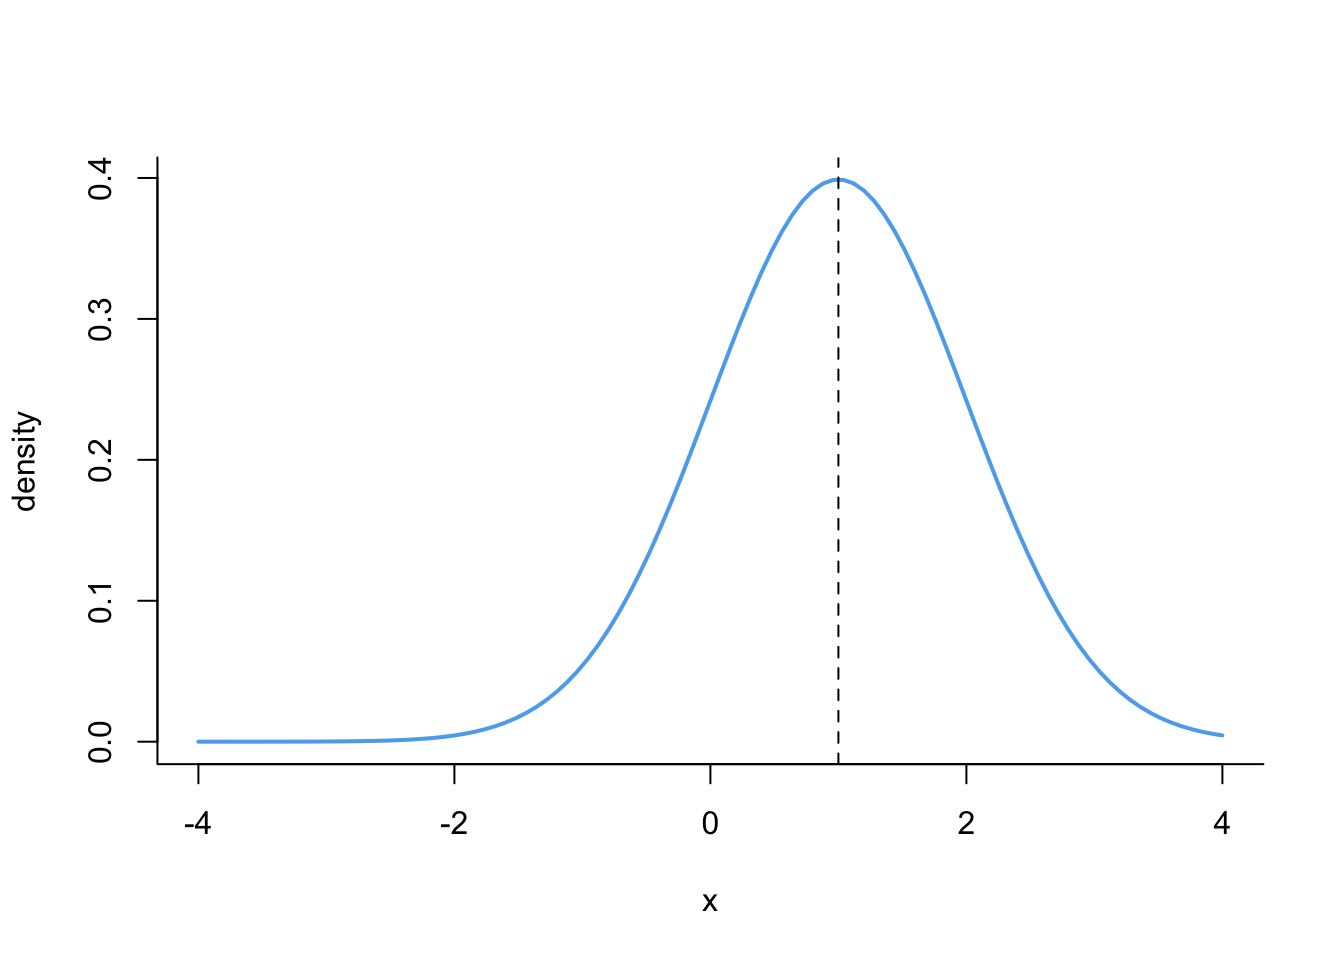
\includegraphics{contRV_files/figure-pdf/fig-norm.dist-1.pdf}

}

\caption{\label{fig-norm.dist-1}Corresponding PMF and CDF}

\end{figure}%

\end{minipage}%
%
\begin{minipage}{0.50\linewidth}

\begin{figure}[H]

\centering{

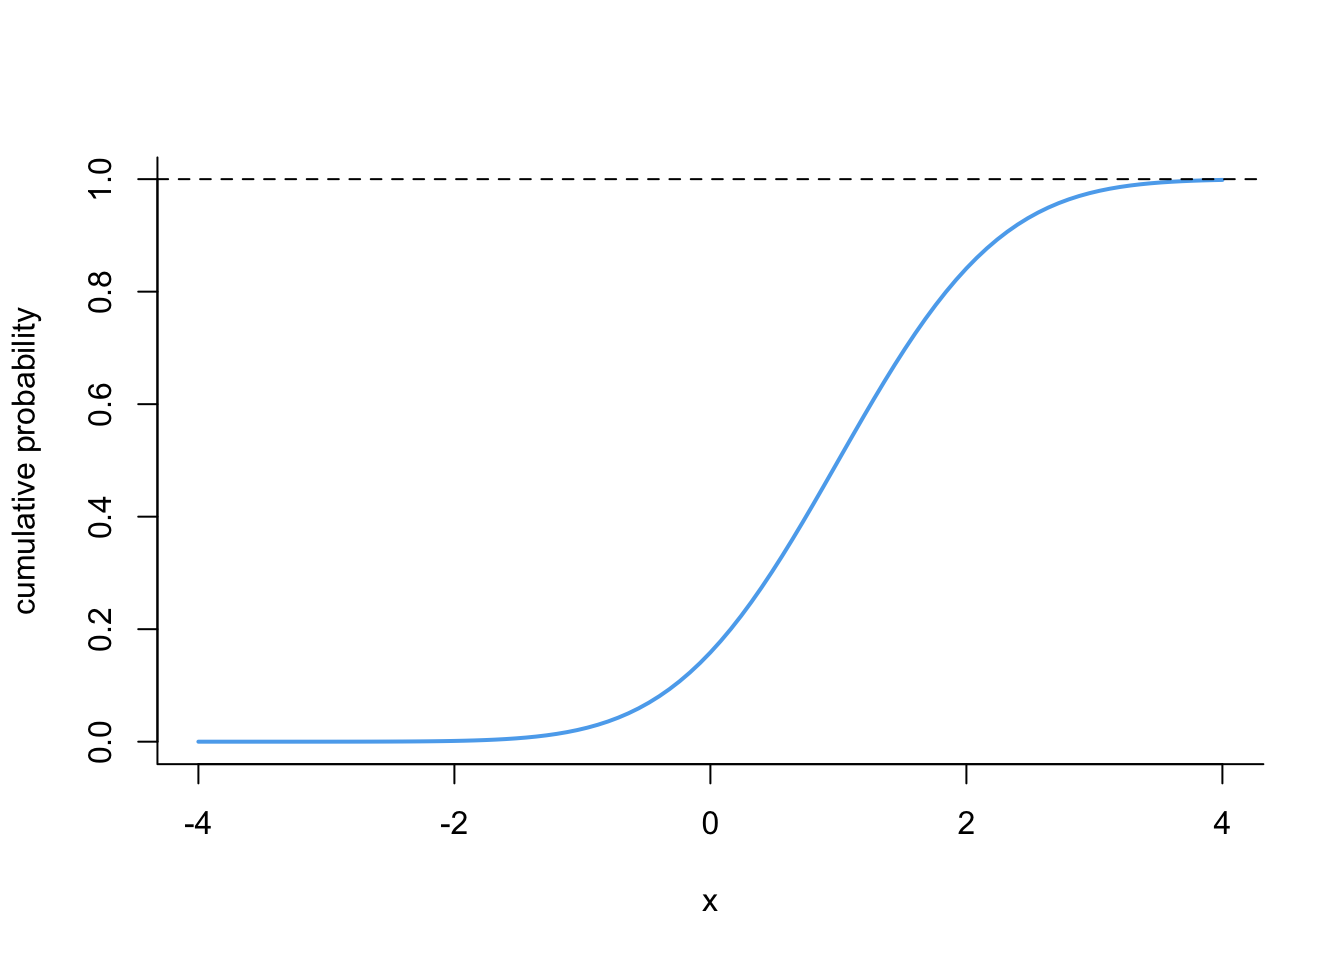
\includegraphics{contRV_files/figure-pdf/fig-norm.dist-2.pdf}

}

\caption{\label{fig-norm.dist-2}Corresponding PMF and CDF}

\end{figure}%

\end{minipage}%

\end{figure}%

\subsubsection{Gamma}\label{gamma}

\part{Generating Random Numbers}

true vs pseudo

Methods to generate random numbers

\begin{enumerate}
\def\labelenumi{\arabic{enumi}.}
\tightlist
\item
  multiplicative congruential random number generator (MCRNG)
\item
  the Inverse Transform Method (ITM)
\item
  a simple method that relies on sample( )
\item
  the acceptance-rejection method (ARM)
\item
  methods to sample from convolutions and from mixture models
\end{enumerate}

\chapter{Multiplicative Congruential Random Number Generator
(MCRNG)}\label{multiplicative-congruential-random-number-generator-mcrng}

(from: Braun and Murdoch's book ``A first course in statistical
programming with R'' 2nd edition (2016): Section 5.2)

\section{Monte Carlo Simulation}\label{monte-carlo-simulation}

to approximate the mean \(\mu = E(x)\): generate m independent and
identically distributed (i.i.d.) values of X and use the sample mean
(\(\bar{X} = \frac{\Sigma X_i}{m}\)) : good approximation for large m
(law of large numbers) the distribution of \(\bar{X}\) can be
approximated by a normal distribution the mean \(\mu\) and variance
\(\sigma ^2 /m\) -\textgreater{} central limit theorem

A multiplicative congruential random number generator (MCRNG) is an
algorithm that can be used to draw numbers from \(X \sim U(0, 1)\)

m large integer, b is another integer where m\textgreater b \(x_0\)
integer between 1 and m \textless- seed

formula \(x_n = bx_{n-1}\)(mod m), \$ u\_n = x\_n / m\$

\begin{verbatim}
 [1] 0.71656713 0.24954631 0.92196522 0.57801828 0.41914409 0.09278385
 [7] 0.95882139 0.91727984 0.77213185 0.80667833 0.74867192 0.77157092
[13] 0.71019896 0.15422180 0.52614907 0.49764081 0.59421916 0.20569505
[19] 0.37954928 0.28247600
\end{verbatim}

\begin{itemize}
\tightlist
\item
  choose m so that it is not divizable by b
\end{itemize}

ex 4

\begin{verbatim}
[1] 0.49605698 0.08148008 0.28544716
\end{verbatim}

\begin{enumerate}
\def\labelenumi{(\alph{enumi})}
\setcounter{enumi}{1}
\tightlist
\item
  Compare your results with the true mean, variance, and standard
  deviation
\end{enumerate}

mean = median of uniform distribution is 1/2(a+b) variance:
\(1/12(b-a)^2\) = 1/12 sd = sqrt(var)

\begin{verbatim}
[1] 0.5
\end{verbatim}

\begin{verbatim}
[1] 0.08333333
\end{verbatim}

\begin{verbatim}
[1] 0.2886751
\end{verbatim}

answer the same to 2d.p

\subsubsection{ex 5}\label{ex-5}

5 Simulate 10000 independent observations on a uniformly distributed
random variable on the interval {[}3.7, 5.8{]}. (a) Estimate the mean,
variance, and standard deviation of such a uniform random variable and
compare your estimates with the true values.

\begin{verbatim}
[1] 4.75
\end{verbatim}

\begin{verbatim}
[1] 4.744036
\end{verbatim}

\begin{verbatim}
[1] 0.3675
\end{verbatim}

\begin{verbatim}
[1] 0.3401287
\end{verbatim}

\begin{verbatim}
[1] 0.6062178
\end{verbatim}

\begin{verbatim}
[1] 0.5832055
\end{verbatim}

\begin{enumerate}
\def\labelenumi{(\alph{enumi})}
\setcounter{enumi}{1}
\tightlist
\item
  Estimate the probability that such a random variable is greater than
  4.0. Compare with the true value.
\end{enumerate}

\begin{verbatim}
[1] 0.888
\end{verbatim}

\begin{verbatim}
[1] 0.8571429
\end{verbatim}

\subsection{Steps}\label{steps}

\begin{itemize}
\item
  draw a sample \(x\) with replacement from a discrete uniform with
  \(\Omega = \{1, 2, ..., k\}\) where \(k \to \infty\), then set
  \(u = \frac{x}{k}\)
\item
  obvious issue: \(k \to \infty\)? (\(\Rightarrow\) choose \(k\) based
  on desired level of accuracy)
\end{itemize}

\subsubsection{Lecture 1 practical}\label{lecture-1-practical}

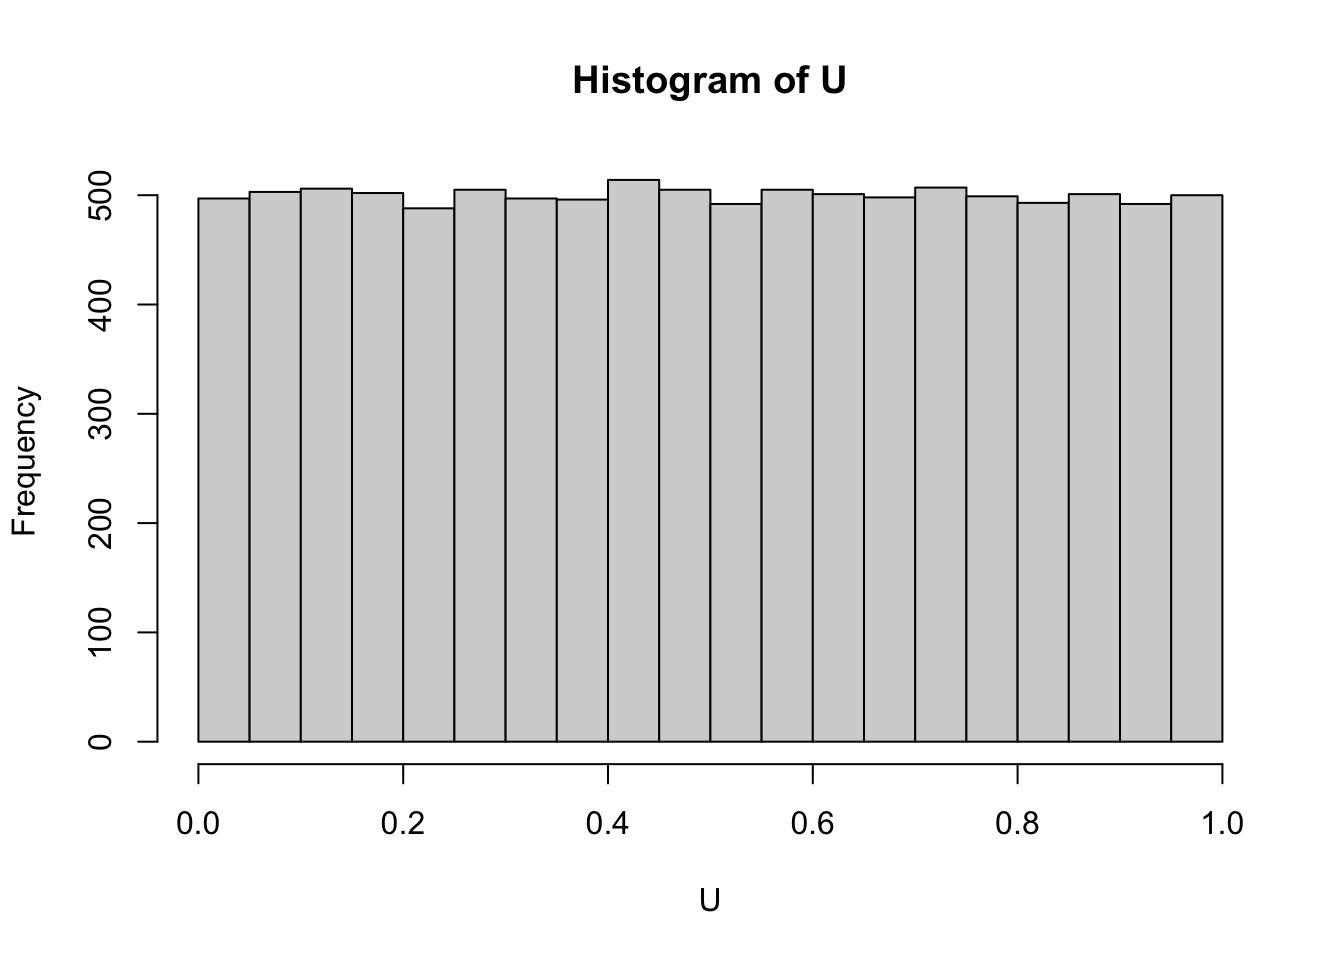
\includegraphics{mcrng_files/figure-pdf/unnamed-chunk-7-1.pdf}

The pseudo-randomly generated numbers u1, . . . , un are approximately
evenly distributed over the interval {[}0, 1{]}. Also, the sample mean
and sample variance of the generated numbers are very close to the
theoretical mean and variance of a U(0, 1)-distributed random variable,
which are 1/2 and 1 12 = 0.083, respectively. This suggests that the
MCRNG algorithm that we implemented is doing a good job at generating
U(0, 1)-distributed random numbers.

\section{Simulation of other random
variables}\label{simulation-of-other-random-variables}

from book

\subsection{Bernoulli random
variables}\label{bernoulli-random-variables}

Write an R function which simulates the outcomes of a student guessing
at a True--False test consisting of n questions. (a) Use the function to
simulate one student guessing the answers to a test with 10 questions;
calculate the number of correct answers for this student. (b) Simulate
the number of correct answers for a student who guesses at a test with
1000 questions.

\begin{verbatim}
[1] 3
\end{verbatim}

\begin{verbatim}
[1] 485
\end{verbatim}

3 Write an R function which simulates 500 light bulbs, each of which has
probability 0.99 of working. Using simulation, estimate the expected
value and variance of the random variable X, which is 1 if the light
bulb works and 0 if the light bulb does not work. What are the
theoretical values?

\begin{verbatim}
[1] 495
\end{verbatim}

\begin{verbatim}
[1] 0.99
\end{verbatim}

\begin{verbatim}
[1] 0.00991984
\end{verbatim}

theoretical values: expectation per bulb = 0.99 and variance is =
p\emph{q (prob of success } prop of fail) = 0.99*0.01

\subsection{Binomial random variables}\label{binomial-random-variables}

Compute the probability of getting four heads in six tosses of a fair
coin

\begin{verbatim}
[1] 0.234375
\end{verbatim}

1 Suppose the proportion defective is 0.15 for a manufacturing
operation. Simulate the number of defectives for each hour of a 24-hour
period, assuming 25 units are produced each hour. Check whether the
number of defectives ever exceeds 5. Repeat, assuming p = 0.2 and then p
= 0.25

\begin{verbatim}
[1] TRUE
\end{verbatim}

\begin{verbatim}
[1] TRUE
\end{verbatim}

\begin{verbatim}
[1] TRUE
\end{verbatim}

Use simulation to estimate the mean and variance of a binomial random
variable with n = 18 and p = 0.76. Compare with the theoretical values.

\begin{verbatim}
[1] 13.689
\end{verbatim}

\begin{verbatim}
[1] 3.059338
\end{verbatim}

theoretical

\begin{verbatim}
[1] 13.68
\end{verbatim}

\begin{verbatim}
[1] 3.2832
\end{verbatim}

The following function simulates binomial pseudorandom numbers by
summing up the corresponding independent Bernoulli random variables.

\subsection{Poisson random variables}\label{poisson-random-variables}

\chapter{Inverse Transform Method
(ITM)}\label{inverse-transform-method-itm}

Two requirements to use the Inverse Transform Method (ITM) to generate
from a random variable \(X\) with cdf \(F_X(x)\):

\begin{enumerate}
\def\labelenumi{\arabic{enumi}.}
\item
  a uniform random number generator \texttt{runif(\ )}
\item
  the inverse cdf, \(F^{−1}_X(p)\)
\end{enumerate}

\begin{tcolorbox}[enhanced jigsaw, bottomrule=.15mm, leftrule=.75mm, colbacktitle=quarto-callout-tip-color!10!white, toptitle=1mm, opacityback=0, titlerule=0mm, colback=white, title=\textcolor{quarto-callout-tip-color}{\faLightbulb}\hspace{0.5em}{Steps}, opacitybacktitle=0.6, left=2mm, rightrule=.15mm, breakable, bottomtitle=1mm, arc=.35mm, coltitle=black, toprule=.15mm, colframe=quarto-callout-tip-color-frame]

\begin{enumerate}
\def\labelenumi{\arabic{enumi}.}
\item
  Compute the inverse of \(F_X(p):F^{−1}_X(p)\)
\item
  Write an \texttt{R} function that computes \(F^{−1}_X(p)\)
\item
  Draw \(u \sim U(0, 1)\) and set \(F^{−1}_X(u)\)
\end{enumerate}

\end{tcolorbox}

\subsubsection{Note}\label{note}

\begin{itemize}
\item
  for a discrete distribution computing the CDF is not difficult: add up
  the individual probabilities for the points of the distribution
\item
  CDF for continuous dist. integrate the PDF
\end{itemize}

\subsection{Example: exponential dist}\label{example-exponential-dist}

\textbf{Step 1}: find the inverse \(F_X(p)\), the cdf is:
\(F_x = 1- exp(-\lambda x)\) for inverse solve:

\[
F_x() = p  \\
F_x() = 1- e^{(-\lambda x)} = p \\
e^{(-\lambda x)} = 1 - p \\
ln(e^{(-\lambda x)}) = ln(1-p) \\
-\lambda x = ln(1-p) \\
x = - \frac{1}{\lambda} \cdot ln(1-p)
\]

\textbf{Step 2 \&3:}

\begin{figure}

\centering{

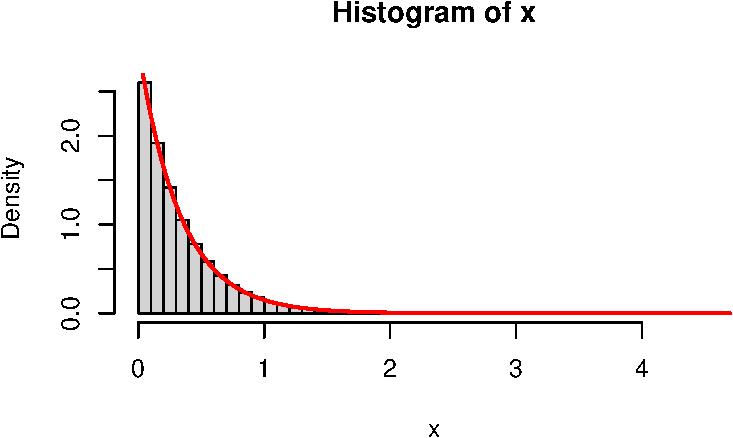
\includegraphics{itm_files/figure-pdf/fig-exp.ex-1.pdf}

}

\caption{\label{fig-exp.ex}Mean = \texttt{r\ mean(x)} and variance
\texttt{r\ var(x)} E(X) if X\textasciitilde exp is 1/lam and var(x)
should be 1/(lam\^{}2)}

\end{figure}%

\subsection{Lecture 1: Exercise 2}\label{lecture-1-exercise-2}

\subsubsection{Step 1: pdf, cdf and expected
value}\label{step-1-pdf-cdf-and-expected-value}

X \textasciitilde{} continuous random variable with density
\(f_X(x) = x^3\) for 0\textless=x\textless=k

\begin{enumerate}
\def\labelenumi{\arabic{enumi}.}
\tightlist
\item
  find k such that \(f_X(x)\) is a pdf
\end{enumerate}

\begin{itemize}
\tightlist
\item
  integrate the pdf
\end{itemize}

\[
\int_{0}^{k} x^3 dx \\
\left[ \frac{x^4}{4} \right]_0^k \\ 
\frac{k^4}{4}- 0 = 1 \\
k^4 = 1*4 \\
k = \sqrt{2}
\]

\begin{enumerate}
\def\labelenumi{\arabic{enumi}.}
\setcounter{enumi}{1}
\tightlist
\item
  Compute the cdf FX(x)
\end{enumerate}

The cdf is the integral of the pdf over it's range

\[
F_X(x)= \int_{0}^{x} f_X(s) ds \\
= \int_{0}^{x} s^3 ds \\
= \frac{x^4}{4}, \text{ when } 0<=x<=k = \sqrt{2}   \\ 
\]

Therefore the cdf is given by:

\[
F_X(x) = 
\begin{cases} 
0, & \text{if  } x < 0; \\
\frac{1}{4}x^4, & \text{if  } 0 \leq x \leq \sqrt{2}; \\
1, & \text{if  } x > \sqrt{2}.
\end{cases}
\]

\begin{enumerate}
\def\labelenumi{\arabic{enumi}.}
\setcounter{enumi}{2}
\tightlist
\item
  Compute E(X)
\end{enumerate}

\[
E(X) = \int_{-\infty}^{\infty} x f_X(x) dx \\
E(X) = \int{0}^{k} x \cdot x^3 dx = \int{0}^{k} x^4 dx\\
E(X) = \left[ \frac{x^5}{5} \right]_0^k \\
E(X) = \left[ \frac{x^5}{5} \right]_0^{\sqrt 2} \\
E(X) = \left[ \frac{(\sqrt 2)^5}{5} \right] - 0 \\
E(X) = \frac{1}{5}(\sqrt 2)^4 (\sqrt 2) \\ 
E(X) = \frac{4}{5}(\sqrt 2)
\]

3.2 Compute Var(X) \(Var(X) = E[X^2] -E[X]^2\)

Step 1

\[
E(X^2) = \int{0}^{k} x2\cdot x3 dx \\
= \int{0}^{k} x^5 dx \\
= \left[ \frac{x^6}{6} \right]_0^k \\
= \left[ \frac{(\sqrt 2)^6}{6} \right] - 0 \\
= \frac{8}{6} = \frac{4}{3} 
\]

Step 2 \([E(X)]^2 = (\frac{4}{5}(\sqrt 2))^2\)

\[
Var(X) = \frac{4}{3} - (\frac{4}{5}(\sqrt 2))^2 = \frac{4}{75}
\]

\subsubsection{Step 2: application of the
ITM}\label{step-2-application-of-the-itm}

Apply the ITM to generate (pseudo)-random numbers from this random
variable:

\textbf{Step 1} Compute the inverse cdf \(F^{−1}_X (x)\)

For \(0<=x<=k = \sqrt{2}\): cdf: \(F_X^{-1}(x) = \frac{x^4}{4}\)

Set \(F_X^{-1}(x) = p\) :

\[
\frac{x^4}{4} = p \ x^4 = 4p \ x = (4p)^{1/4} \\
F_X^{-1}(p) = (4p)^{1/4}
\]

and (b) write an R function to generate random numbers from X ∼ fX(x)
that relies on the ITM.

\subsubsection{Step 3: double-check your random number
generator}\label{step-3-double-check-your-random-number-generator}

\begin{enumerate}
\def\labelenumi{\arabic{enumi}.}
\setcounter{enumi}{7}
\tightlist
\item
  Compare the range of the numbers generated at point (7) to the support
  of X. What do you notice?
\end{enumerate}

\begin{verbatim}
   Min. 1st Qu.  Median    Mean 3rd Qu.    Max. 
 0.1127  0.9983  1.1889  1.1323  1.3166  1.4142 
\end{verbatim}

The support of X is (\(0, \sqrt2\)) but the range of the sample is
(0.11, 1.4).

\begin{enumerate}
\def\labelenumi{\arabic{enumi}.}
\setcounter{enumi}{8}
\tightlist
\item
  Compute the mean and variance of the numbers generated at point (7),
  and compare them to the values of E(X) and V ar(X) that you computed
  at point (3). Are the numerical results in agreement with your
  analytical derivations?
\end{enumerate}

\begin{verbatim}
[1] 1.132304
\end{verbatim}

\begin{verbatim}
[1] 0.05234072
\end{verbatim}

analytical:

\begin{verbatim}
[1] 1.333333
\end{verbatim}

\begin{verbatim}
[1] 0.05333333
\end{verbatim}

\begin{enumerate}
\def\labelenumi{\arabic{enumi}.}
\setcounter{enumi}{9}
\tightlist
\item
  Draw a histogram that shows the empirical density of the 10000 random
  numbers, and compare it to fX(x)
\end{enumerate}

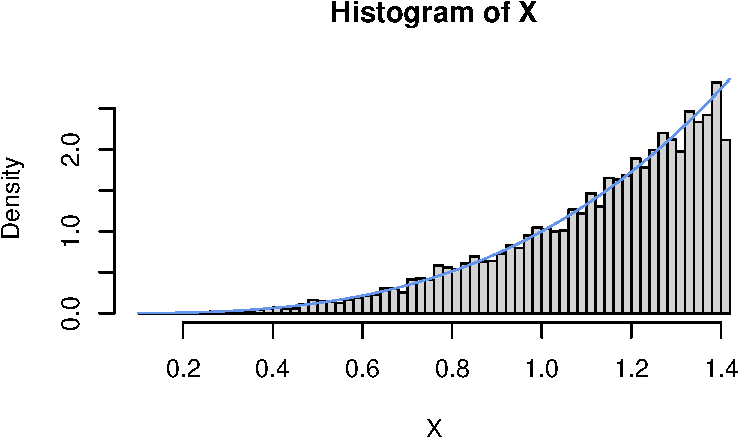
\includegraphics{itm_files/figure-pdf/unnamed-chunk-8-1.pdf}

The values generated are close to the curve of \(f_X(x)\)

\chapter{(lecture 2) Discrete R.V.}\label{lecture-2-discrete-r.v.}

\subsubsection{Example: binomial
distribution}\label{example-binomial-distribution}

\begin{verbatim}
 [1] 3 4 4 3 5 5 3 1 2 2
\end{verbatim}

\begin{verbatim}
  omega     pmf rel.freq
1     0 0.02799  0.02832
2     1 0.13064  0.13305
3     2 0.26127  0.25915
4     3 0.29030  0.29070
5     4 0.19354  0.19191
6     5 0.07741  0.07758
7     6 0.01720  0.01763
8     7 0.00164  0.00166
\end{verbatim}

\begin{itemize}
\item
  sample(1:k, n, replace = T, prob = c(\ldots)) allows you to generate n
  independent realizations from a multinomial distribution
\item
  each single draw from sample( ) as an application of the ITM
\end{itemize}

\subsubsection{Example}\label{example}

\(\Omega = {1, 2, 3, 4}\), \(P(X = k) = \frac{k}{10}\) for
\(\Omega \in k\)

\begin{enumerate}
\def\labelenumi{\arabic{enumi}.}
\item
  pdf: \(P(X = k) = \frac{k}{10}\) Where k can be 1,\ldots4
\item
  cdf is defined as \(F_X(x) = P(X <= k)\) i.e.~the sum of probabilities
  of all the outcomes of k.
\end{enumerate}

\[
F_X(x) =
\begin{cases} 
0                                         &  x < 1; \\
\frac{1}{10}                              & 1 \leq x \leq{2} 
                                                \text{ i.e.  }P(X=1); \\
\frac{1}{10}+\frac{2}{10} = \frac{3}{10}  & 2 \leq x \leq{3}; \\
\frac{6}{10}                              & 3 \leq x \leq{4}; \\
1                                         &  x <4; \\
\end{cases}
\]

\paragraph{Applying ITM}\label{applying-itm}

\begin{itemize}
\tightlist
\item
  Draw from a U(0, 1)\\
\item
  Apply the inverse CDF to determine the outcome
\end{itemize}

Suppose we generate u1 = 0.55 This u is in the interval of
\(\frac{3}{10}\leq x < \frac{6}{10}\) The corresponding value of X for
this interval is 3 Therefore \(F_X^{-1}(0.55) =3\)

\cleardoublepage
\phantomsection
\addcontentsline{toc}{part}{Appendices}
\appendix

\chapter{How I made this}\label{how-i-made-this}

\section{Github}\label{github}

https://happygitwithr.com/

\section{git website}\label{git-website}

https://www.codecademy.com/article/creating-a-website-on-github-pages

\section{\texorpdfstring{\textbf{quarto-webr}}{quarto-webr}}\label{quarto-webr}

https://quarto-webr.thecoatlessprofessor.com/

\section{Inspiration}\label{inspiration}

https://dkon1.github.io/quant\_life\_quarto/tutorial3.html

https://github.com/casrou/ProbToPdf/blob/master/Introduction\%20to\%20Probability\%2C\%20Statistics\%2C\%20and\%20Random\%20Processes\%20-\%20Hossein\%20Pishro-Nik.pdf

\phantomsection\label{refs}
\begin{CSLReferences}{1}{0}
\bibitem[\citeproctext]{ref-pishro-nik2014}
Pishro-Nik, Hossein. 2014. \emph{Introduction to Probability,
Statistics, and Random Processes}. Blue Bell, PA: Kappa Research, LLC.

\end{CSLReferences}



\end{document}
